\bookchapter{Bab 42: Panorama Model Bahasa Besar dan Praktik API}

\chapterintro{Bab-bab sebelum ini bercakap tentang “cara bekerjasama dengan AI”; bab ini menyelesaikan satu soalan yang lebih asas: “gunakan AI yang mana? bagaimana menggunakannya?” Landskap model bahasa besar pada Ogos 2026 sudah sangat pelbagai — di peringkat antarabangsa ada pertarungan tiga kuasa besar iaitu GPT, Claude dan Gemini; di China pula ada DeepSeek, Tongyi Qianwen, GLM, Kimi dan Doubao yang berkembang masing-masing. Setiap model mempunyai personaliti dan kepakaran tersendiri: pilih dengan tepat, kerja menjadi lebih mudah; pilih dengan salah, kerja menjadi lebih sukar. Bab ini bukan sahaja membawa anda mengenali model-model ini, malah mengajar anda cara menyambungkannya ke aplikasi anda sendiri melalui API, serta cara memilih Token Plan (pakej penggunaan) yang sesuai mengikut keperluan anda.}

\booksection{Model Bahasa Besar Antarabangsa Utama: Landskap Tiga Kuasa}

Pasaran model bahasa besar antarabangsa pada Ogos 2026 telah membentuk landskap tiga kuasa besar: OpenAI (siri GPT), Anthropic (siri Claude) dan Google (siri Gemini). Setiap syarikat mempunyai ciri yang tersendiri — mari kita kenali satu demi satu.

\booksubsection{Siri OpenAI GPT-5.6: Pejuang Serba Boleh yang Seimbang}

OpenAI ialah perintis gelombang model bahasa besar, dan siri GPT sehingga kini masih menjadi model paling luas digunakan di dunia. Siri GPT-5.6 yang dikeluarkan pada Julai 2026 menggunakan strategi tiga kedudukan: varian utama GPT-5.6 Sol untuk keperluan penaakulan tahap tinggi, varian seimbang GPT-5.6 Terra untuk pembangunan harian, dan varian ringan GPT-5.6 Luna untuk senario beban serentak tinggi berkos rendah. Ketiga-tiga model berkongsi tetingkap konteks 1.05 juta Token, dan semuanya menyokong input imej, pemanggilan fungsi serta output berstruktur.

\begin{center}
\begin{tabularx}{\linewidth}{|X|X|X|X|X|}
\hline
\textbf{Varian} & \textbf{Peranan} & \textbf{Input (/juta Token)} & \textbf{Output (/juta Token)} & \textbf{Tetingkap konteks} \tabularnewline
\hline
GPT-5.6 Sol & Penaakulan utama & US\$5.00 (sekitar 36 yuan) & US\$30.00 (sekitar 217 yuan) & 1.05 juta Token \tabularnewline
GPT-5.6 Terra & Seimbang harian & US\$2.50 (sekitar 18 yuan) & US\$15.00 (sekitar 109 yuan) & 1.05 juta Token \tabularnewline
GPT-5.6 Luna & Ringan kos rendah & US\$1.00 (sekitar 7 yuan) & US\$6.00 (sekitar 44 yuan) & 1.05 juta Token \tabularnewline
\hline
\end{tabularx}
\end{center}

\begin{center}\small\color{gray}Harga siri OpenAI GPT-5.6 (Ogos 2026)\end{center}

Kelebihan teras siri GPT terletak pada “keseimbangan” — penaakulan, pengaturcaraan, penulisan, multimodal; tiada kelemahan yang ketara. Ditambah pula dengan ekosistem sambungan OpenAI yang besar dan komuniti pembangunnya, dokumentasi dan rantaian alatnya paling lengkap. Bagi senario “tidak tahu nak pilih apa”, GPT ialah jawapan lalai “pilih dengan mata tertutup pun tidak silap”. Tetapi kelemahannya: akses dari China memerlukan rangkaian khas, ungkapan bahasa Cinanya kadangkala berbau “terjemahan”, dan harga API berada pada tahap sederhana hingga tinggi.

\textbf{Berita Baik}\par

Pada Ogos 2026, OpenAI mengumumkan model lalai untuk pengguna percuma dinaik taraf kepada GPT-5.6 Luna, serta membuka sembang teks tanpa had. Ini bermakna anda boleh merasai keupayaan asas GPT tanpa kos; bayaran hanya diperlukan apabila anda memerlukan penaakulan yang lebih kuat atau panggilan API.

\booksubsection{Siri Anthropic Claude: Puncak Pengaturcaraan dan Kejituan}

Jika GPT ialah atlet serba boleh, maka Claude ialah “puncak” dalam bidang pengaturcaraan. Siri Claude daripada Anthropic mendahului SWE-bench (ujian penanda aras kejuruteraan perisian) secara berterusan dengan jurang yang jauh, dengan kualiti penjanaan kod dan keupayaan melaksanakan projek peringkat kejuruteraan yang terbaik dalam industri. Lebih jarang lagi, kadar halusinasi Claude (kebarangkalian menjana maklumat palsu) paling rendah di seluruh rangkaian, hanya sekitar 1\% — menjadikannya sangat sesuai untuk senario ketepatan tinggi seperti akademik dan undang-undang.

Senjata maut Claude yang satu lagi ialah konteks jangka panjang luar biasa: menyokong tetingkap konteks 1 juta Token, mampu “membaca habis” kontrak beratus-ratus muka surat atau seluruh kod projek sekali gus tanpa terlepas butiran. Ini hampir tiada pengganti dalam senario seperti penstrukturan semula kod dan analisis dokumen panjang. Claude Code, sebagai alat pengaturcaraan AI terminal, mencapai pendapatan tahunan AS\$2.5 bilion menjelang pertengahan 2026 — itulah bukti paling kukuh pengiktirafan terhadap keupayaan pengaturcaraan Claude.

\begin{center}
\begin{tabularx}{\linewidth}{|X|X|X|X|X|}
\hline
\textbf{Varian} & \textbf{Peranan} & \textbf{Input (/juta Token)} & \textbf{Output (/juta Token)} & \textbf{Tetingkap konteks} \tabularnewline
\hline
Claude Fable 5 & Varian utama & US\$10.00 (sekitar 72 yuan) & US\$50.00 (sekitar 362 yuan) & 1 juta Token \tabularnewline
Claude Opus 4.8 & Varian profesional & US\$5.00 (sekitar 36 yuan) & US\$25.00 (sekitar 181 yuan) & 1 juta Token \tabularnewline
Claude Sonnet 5 & Varian nilai wang & US\$2.00 (sekitar 14 yuan) & US\$10.00 (sekitar 72 yuan) & 1 juta Token \tabularnewline
\hline
\end{tabularx}
\end{center}

\begin{center}\small\color{gray}Harga siri Anthropic Claude (Ogos 2026; Sonnet 5 pada harga diskaun)\end{center}

Kelemahan Claude ialah harga — harga output Fable 5 paling tinggi antara semua model, iaitu AS\$50 setiap juta Token. Keupayaan multimodalnya (kefahaman imej dan video) juga agak lemah. Bagi pembangun persendirian berkemampuan terhad, Sonnet 5 pada tempoh diskaun sangat menonjol dari segi nilai wang.

\booksubsection{Siri Google Gemini: Raja Multimodal}

Siri Gemini daripada Google telah berkembang ke versi 3.1 Pro pada 2026. Senjata maut terbesar Gemini ialah multimodal asli — penghuraian imej dan teks yang tepat, pengesanan jadual OCR tanpa ralat, pengekstrakan bingkai video yang cekap, dan turut menyokong penghuraian audio dan video secara mendalam. Ia terikat rapat dengan ekosistem Google (carian, e-mel, perkhidmatan awan) dan menonjol dalam pengambilan maklumat masa nyata serta kefahaman merentas modal. Gemini turut menyokong input konteks sehingga 2 juta Token, iaitu tetingkap konteks terbesar pada masa kini.

Kedudukan Gemini ialah “pilihan utama bagi penaakulan saintifik dan senario multimodal”. Jika projek anda melibatkan banyak analisis imej, kefahaman video atau pengiraan saintifik, Gemini hampir tiada penanding. Tetapi dalam penjanaan kod teks tulen ia sedikit kalah daripada Claude, dan ungkapan bahasa Cinanya juga tidak semula jadi seperti model buatan China.

\begin{center}
\begin{tabularx}{\linewidth}{|X|X|X|X|}
\hline
\textbf{Perkara perbandingan} & \textbf{GPT-5.6} & \textbf{Claude Fable 5} & \textbf{Gemini 3.1 Pro} \tabularnewline
\hline
Skor keseluruhan & 94.8 & 95.0 & 92.1 \tabularnewline
Keupayaan pengaturcaraan (SWE-bench) & 74.9\% & 64.3\% (Pro) & Sederhana \tabularnewline
Tetingkap konteks & 1.05 juta Token & 1 juta Token & 2 juta Token \tabularnewline
Keupayaan multimodal & Seimbang & Agak lemah & Paling kuat \tabularnewline
Kadar halusinasi & Agak rendah & Paling rendah (sekitar 1\%) & Agak rendah \tabularnewline
Ketersediaan di China & Perlu rangkaian khas & Perlu rangkaian khas & Perlu rangkaian khas \tabularnewline
Ekosistem API & Paling lengkap & Sedang berkembang & Terikat pada ekosistem Google \tabularnewline
\hline
\end{tabularx}
\end{center}

\begin{center}\small\color{gray}Perbandingan mendatar tiga model antarabangsa (Ogos 2026)\end{center}

\begin{tcbwarn}{Perhatian: Halangan realiti penggunaan di China}
Bagi pembangun di China, halangan utama GPT, Claude dan Gemini ialah akses rangkaian. Walaupun boleh digunakan secara tidak langsung melalui proksi Azure, platform agregasi API dan sebagainya, kestabilan dan pematuhan perlu dinilai sendiri. Jika projek anda mempunyai keperluan ketat terhadap keselamatan data, disyorkan mengutamakan model buatan China.

\end{tcbwarn}

\booksection{Model Bahasa Besar Buatan China Utama: Pelbagai Jenis Berkembang}

Pada 2026, model bahasa besar buatan China telah bertukar daripada “pengejar” kepada “pelari seiring”, malah “mendahului” dalam sesetengah bidang. Berbeza dengan kontroversi “model pembalut” tahun 2023, model utama buatan China pada 2026 sudah setanding dengan model tahap terbaik antarabangsa dalam penaakulan logik, penjanaan kod dan kefahaman bahasa Cina, dengan jurang menyusut kepada bawah 5\%. Lebih penting lagi, model buatan China mempunyai kelebihan yang tidak boleh digantikan dalam senario bahasa Cina, kos harga dan pelancaran yang mematuhi peraturan.

\booksubsection{DeepSeek V4: Raja Nilai Wang}

DeepSeek ialah kehadiran fenomena dalam kalangan model bahasa besar buatan China. Pada awal 2025, DeepSeek-V3 menggemparkan pasaran dengan kedudukan “sepuluh kali lebih murah daripada GPT tetapi keupayaan setanding”, dan digelar industri sebagai “garis pemusnah” model AI sejagat — yang lebih murah tidak sebaik ia, yang lebih mahal pula tidak selimpat ia. Menjelang Ogos 2026, versi rasmi DeepSeek V4-Pro dikeluarkan: seni bina MoE berskala 1.6 trilion parameter dengan pengaktifan sekitar 49B, menyokong konteks 1 juta tanpa kehilangan, dan nilai wangnya bagi kod secara meluas dianggap puncak dunia.

DeepSeek V4 mencapai lompatan besar dalam keupayaan Agent — penanda aras DeepSWE melonjak daripada 12.8 kepada 62.7 (+390\%), dan NL2Repo meningkat daripada 38.5 kepada 61.5. API menambah sokongan dwi-protokol Responses API dan Anthropic API, dan telah serasi dengan alat pengaturcaraan arus perdana seperti Codex dan Claude Code. Ini bermakna anda boleh menggunakan API DeepSeek menggantikan API Claude dalam Claude Code — kos menurun beberapa kali ganda, pengalaman hampir sama.

\begin{center}
\begin{tabularx}{\linewidth}{|X|X|X|X|X|}
\hline
\textbf{Varian} & \textbf{Peranan} & \textbf{Input (/juta Token)} & \textbf{Output (/juta Token)} & \textbf{Tetingkap konteks} \tabularnewline
\hline
DeepSeek V4 Pro & Penaakulan utama & 3 yuan (sekitar US\$0.43) & 6 yuan (sekitar US\$0.87) & 1 juta Token \tabularnewline
DeepSeek V4 Flash & Ringan pantas & 1 yuan (sekitar US\$0.14) & 2 yuan (sekitar US\$0.28) & 1 juta Token \tabularnewline
\hline
\end{tabularx}
\end{center}

\begin{center}\small\color{gray}Harga siri DeepSeek V4 (Ogos 2026, harga promosi)\end{center}

Perbandingan harga: bagi 1 juta Token input + 1 juta Token output yang sama, DeepSeek V4 Flash berkos sekitar AS\$0.42, GPT-5.6 Sol sekitar AS\$35, dan Claude Fable 5 sekitar AS\$60. Jurangnya sehingga 80-140 kali ganda.

\textbf{Peringatan elak jerat: Harga DeepSeek akan naik}\par

Pihak rasmi DeepSeek telah mengumumkan pada 6 Ogos 2026 “berancangan menaikkan harga API secara besar-besaran dalam masa terdekat”, jadi harga promosi mungkin tidak bertahan lama. Sebahagian media mengkhabarkan kenaikan mungkin mencapai 30 kali ganda; sehingga 14 Ogos, pihak rasmi masih belum mengumumkan pelan penetapan harga akhir. Selain itu, versi rasmi DeepSeek V4 memperkenalkan mekanisme harga puncak dan lembah — harga panggilan pada waktu puncak meningkat dua kali ganda. Disyorkan memantau pengumuman rasmi untuk harga terkini.

\booksubsection{Tongyi Qianwen Qwen3.7 Max: Pilihan Peringkat Perusahaan Alibaba Cloud}

Siri Tongyi Qianwen (Qwen) daripada Alibaba Cloud bersandar pada ekosistem Alibaba Cloud dan mempunyai kelebihan semula jadi dalam pelancaran peringkat perusahaan. Qwen3.7 Max yang dikeluarkan pada Julai 2026 ialah model utama semasa: model padat 235B parameter dengan konteks asli 256K, boleh dikembangkan sehingga 1M. Kelebihan teras Qwen: ekosistem sumber terbuka yang matang (seluruh siri daripada 7B hingga 235B bersumber terbuka), kefahaman senario bahasa Cina yang tepat, serta integrasi mendalam dengan infrastruktur Alibaba Cloud.

\begin{center}
\begin{tabularx}{\linewidth}{|X|X|X|}
\hline
\textbf{Varian} & \textbf{Harga output (/juta Token)} & \textbf{Senario sesuai} \tabularnewline
\hline
qwen-turbo & 0.6 yuan & Soal jawab minimum, pengelasan teks, beban serentak tinggi \tabularnewline
qwen-long & 2.0 yuan & Pemprosesan konteks amat panjang 10M \tabularnewline
qwen3.7-flash & 7.2 yuan & Sembang umum, penjanaan kandungan \tabularnewline
qwen3.7-plus & 12.0 yuan & Multimodal (imej + video), penulisan bahasa Cina \tabularnewline
qwen3.7-max & 36.0 yuan & Keupayaan bahasa Cina tahap utama, tugasan kompleks \tabularnewline
\hline
\end{tabularx}
\end{center}

\begin{center}\small\color{gray}Harga berperingkat siri Tongyi Qianwen Qwen (Ogos 2026)\end{center}

Harga Qwen menggunakan strategi berperingkat — daripada qwen-turbo berkos sangat rendah (output 0.6 yuan/juta Token) hingga model utama qwen3.7-max (output 36 yuan/juta Token), meliputi keseluruhan keperluan daripada soal jawab ringan hingga penaakulan kompleks. Bagi perusahaan yang sudah menggunakan Alibaba Cloud, Qwen ialah pilihan integrasi paling mudah.

\booksubsection{Zhipu GLM-5.1: Yang Pertama SWE-bench Buatan China}

Siri GLM daripada Zhipu AI mempamerkan prestasi cemerlang pada 2026. GLM-5.1 meraih keputusan pertama buatan China pada SWE-bench: seni bina hibrid padat MoE 744B, menyokong konteks 1 juta. Kepakarannya ialah kefahaman semantik bahasa Cina yang tepat, serta menyokong pelancaran peribadi yang mematuhi peraturan di China — ini sangat penting bagi senario kewangan dan kerajaan yang menuntut keselamatan data tinggi. Harga GLM-5.1 ialah 6 yuan untuk input dan 24 yuan untuk output setiap juta Token, berada pada tahap pertengahan model buatan China.

\booksubsection{Kimi K3: Raja Teks Jangka Panjang}

Siri Kimi daripada Moonshot AI terkenal dengan keupayaan memproses teks jangka panjang luar biasa. Kimi K3 yang dikeluarkan pada Julai 2026 berskala 2.8 trilion parameter dan memasuki gred pertama dunia dalam banyak penilaian tugasan kompleks. Senario teras Kimi ialah analisis kod sumber panjang dan pengambilan semula dokumen panjang yang dipertingkat — ia boleh memproses teks seluruh buku atau kod seluruh projek, dan cemerlang dalam tugasan pengambilan gaya “mencari jarum dalam timbunan jerami”. Harga Kimi agak tinggi (output sekitar 12-20 yuan/juta Token), tetapi nilai wangnya dalam senario teks panjang tiada penanding.

\booksubsection{Doubao: Atlet Serba Boleh ByteDance}

Siri Doubao daripada ByteDance mempamerkan prestasi stabil pada 2026. Doubao Seed 2.1 Pro ialah model utama Volcengine dengan konteks 256K, prestasi keseluruhan yang stabil dalam ujian sebenar, dan pengalaman senario bahasa Cina yang menonjol. Kelebihan Doubao: pendaftaran terus menerima Token percuma dalam kuantiti banyak, integrasi ekosistem Volcengine yang lengkap, dan harga dalam kalangan yang paling rendah di China. Bagi pemula yang ingin cepat merasai pengaturcaraan AI, Doubao ialah pilihan permulaan tanpa halangan.

\begin{center}
\begin{tabularx}{\linewidth}{|X|X|X|X|X|X|}
\hline
\textbf{Perkara perbandingan} & \textbf{DeepSeek V4} & \textbf{Qwen3.7 Max} & \textbf{GLM-5.1} & \textbf{Kimi K3} & \textbf{Doubao 2.1 Pro} \tabularnewline
\hline
Skor keseluruhan & 87.5 & 89.7 & 90.5 & 88+ & 85+ \tabularnewline
Keupayaan pengaturcaraan & Amat kuat & Kuat & SWE pertama buatan China & Kuat & Pertengahan ke atas \tabularnewline
Kefahaman bahasa Cina & Cemerlang & Cemerlang & Tepat & Cemerlang & Cemerlang \tabularnewline
Tetingkap konteks & 1 juta & 256K-1M & 1 juta & Amat panjang & 256K \tabularnewline
Harga output (yuan/M) & 6 & 36 & 24 & 12-20 & 30 \tabularnewline
Sumber terbuka & Lesen MIT & Seluruh siri sumber terbuka & Sebahagian sumber terbuka & Sumber tertutup & Sumber tertutup \tabularnewline
Pelancaran peribadi & Disokong & Disokong & Disokong & Tidak disokong & Tidak disokong \tabularnewline
\hline
\end{tabularx}
\end{center}

\begin{center}\small\color{gray}Perbandingan mendatar lima model buatan China (Ogos 2026)\end{center}

Satu trend penting: “rasa jurang generasi” antara model buatan China dengan GPT/Claude telah hilang. Dalam penaakulan logik dan pertandingan matematik, jurang skor antara model utama buatan China dengan GPT-5 secara amnya hanya dalam angka satu digit. Dalam pemikiran seni bina berstruktur dan penaakulan kejuruteraan kompleks, Claude masih mendahului — ia mampu memberikan pelan seni bina yang lebih bernyawa dengan kreativiti, manakala model buatan China kadangkala kelihatan “kaku”. Tetapi dalam senario bahasa Cina, kawalan kos dan pelancaran yang mematuhi peraturan, model buatan China mempunyai kelebihan yang jauh mengatasi.

\begin{center}
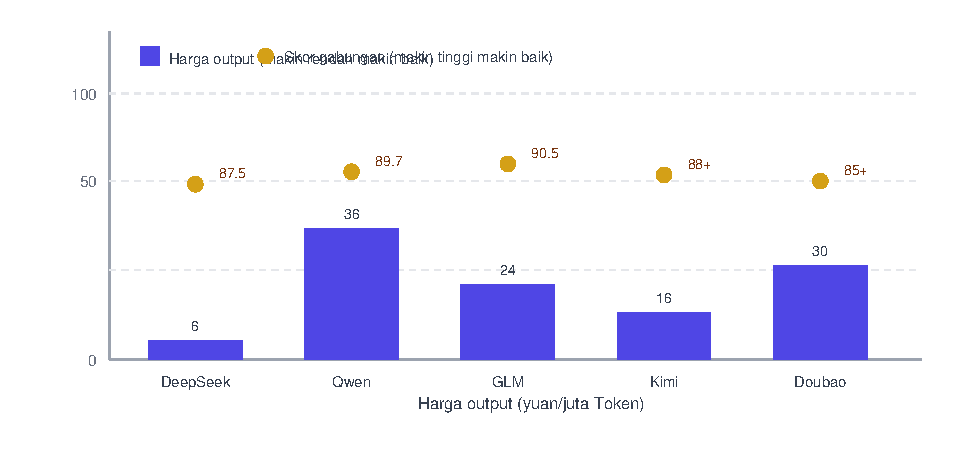
\includegraphics[width=0.92\linewidth]{figures/fig-di-si-shi-er-zhang-1}
\\[2pt]\small Rajah 4: Perbandingan harga dan prestasi lima model (harga semakin rendah semakin baik, skor semakin tinggi semakin baik)
\end{center}

\booksection{Kerangka Keputusan Pemilihan Model}

Selepas memahami ciri setiap model, bagaimana memilih model untuk projek anda? Di sini kami berikan anda “kaedah keputusan empat soalan” — jawab empat soalan ini, dan anda boleh mengunci model yang paling sesuai dengan anda.

Projek anda dilaksanakan dalam negara atau antarabangsa?

Dalam negara pilih model tempatan

|

Antarabangsa boleh pilih model luar negara

Tugas utamanya pengekodan atau lain?

Pengekodan Claude atau DeepSeek

|

Lain-lain terus nilai

Perlu konteks sangat panjang (>500K Token)?

Perlu Gemini atau Kimi

|

Tidak perlu terus nilai

Bajet terhad?

Sensitif DeepSeek atau Qwen-turbo

|

Tidak sensitif GPT-5.6 atau Claude

\begin{center}\small\color{gray}Rajah 5: Kaedah keputusan empat soalan pemilihan model bahasa besar\end{center}

\begin{tcbinfo}{Petua: Strategi gabungan}
Kaedah keputusan ini bukan dogma — banyak senario memerlukan gabungan beberapa model. Satu strategi gabungan yang lazim: guna DeepSeek atau Qwen untuk pembangunan harian (kos rendah, bahasa Cina bagus), Claude untuk reka bentuk seni bina kritikal (penaakulan kuat, halusinasi rendah), dan Gemini untuk analisis multimodal (pemprosesan imej dan video). Tukar model mengikut keperluan, bukan “satu model diguna sehingga tamat”.

\end{tcbinfo}

\booksection{Asas Panggilan API: Menyambungkan Model Bahasa Besar dari Sifar}

Banyak tutorial pengaturcaraan AI hanya mengajar anda menggunakan antara muka sembang, tetapi “pengaturcaraan AI” yang sebenar — membolehkan aplikasi anda memanggil model bahasa besar — perlu melalui API. API (Application Programming Interface, antara muka pengaturcaraan aplikasi) ialah protokol komunikasi antara atur cara. Melalui API, kod anda boleh memanggil keupayaan model bahasa besar seperti memanggil satu fungsi.

\booksubsection{Apakah Itu Token}

Sebelum memahami API, anda mesti memahami konsep “Token” dahulu. Token ialah unit asas pengebilan model bahasa besar, boleh difahami sebagai “unit bacaan dan penulisan AI”. Satu Token lebih kurang bersamaan: 0.75 patah perkataan (4 aksara) dalam bahasa Inggeris, dan 0.5-1 aksara Cina dalam bahasa Cina. Satu teks bahasa Cina sepanjang 1000 aksara mengguna kira-kira 1500-2000 Token.

Token bukan bilangan perkataan, juga bukan bilangan aksara. Model bahasa besar menggunakan peng-token khusus (Tokenizer) untuk memotong teks menjadi Token. Bilangan Token bagi perkataan yang sama mungkin berbeza antara model — contohnya, “kecerdasan buatan” mungkin 3 Token dalam GPT tetapi 2 dalam DeepSeek. API kebanyakan model memulangkan jumlah Token yang sebenarnya digunakan, dan anda boleh melihatnya dalam respons API.

\begin{tcbinfo}{Anggaran Kos Token dengan Pantas}
1 juta aksara bahasa Cina bersamaan kira-kira 1.5 juta Token. Menggunakan DeepSeek V4 Flash untuk 1 juta aksara input + 1 juta aksara output berkos sekitar AS\$0.42 (sekitar 3 yuan); menggunakan Claude Fable 5 untuk kuantiti yang sama berkos sekitar AS\$60 (sekitar 434 yuan). Itulah sebabnya pemilihan model mempengaruhi kos projek anda secara langsung.

\end{tcbinfo}

\booksubsection{Memperoleh API Key}

Langkah pertama menggunakan API model bahasa besar ialah memperoleh API Key — satu rentetan kunci untuk pengesahan identiti. Setiap penyedia model mempunyai platform API tersendiri; anda perlu mendaftar akaun dan mencipta API Key. Berikut ialah pintu masuk platform API model-model utama dan proses memperolehnya:

\begin{center}
\begin{tabularx}{\linewidth}{|X|X|X|X|}
\hline
\textbf{Model} & \textbf{Platform API} & \textbf{Proses perolehan} & \textbf{Kuota percuma} \tabularnewline
\hline
DeepSeek & platform.deepseek.com & Daftar Sahkan identiti Cipta API Key & Kuota hadiah untuk pengguna baharu \tabularnewline
Tongyi Qianwen & bailian.aliyun.com (Platform Bailian) & Log masuk akaun Alibaba Cloud Aktifkan perkhidmatan Cipta Key & Percubaan percuma untuk pengguna baharu \tabularnewline
Zhipu GLM & open.bigmodel.cn & Daftar Sahkan identiti Cipta API Key & Kuota hadiah untuk pengguna baharu \tabularnewline
Kimi & platform.moonshot.cn & Daftar Sahkan identiti Cipta API Key & Kuota percuma terhad \tabularnewline
Doubao & volcengine.com (Volcengine) & Daftar Aktifkan Volcano Ark Cipta API Key & Pendaftaran memberi Token percuma yang banyak \tabularnewline
OpenAI GPT & platform.openai.com & Daftar Ikat kad kredit Cipta API Key & Tiada kuota percuma (perlu bayar) \tabularnewline
Anthropic Claude & console.anthropic.com & Daftar Ikat kad Cipta API Key & Kuota kecil untuk pengguna baharu \tabularnewline
\hline
\end{tabularx}
\end{center}

\begin{center}\small\color{gray}Platform API model utama dan cara memperoleh Key (Ogos 2026)\end{center}

\textbf{Peringatan keselamatan: API Key = kata laluan dompet}\par

API Key setara dengan kata laluan dompet anda — sesiapa yang mendapat Key boleh menggunakan kuota anda untuk memanggil model. Oleh itu: jangan sesekali menulis API Key dalam kod (urus dengan pemboleh ubah persekitaran); jangan sesekali memuat naik kod yang mengandungi Key ke repositori Git awam; jangan sesekali berkongsi tangkapan skrin yang mengandungi Key di media sosial. Jika Key bocor, padamkan serta-merta di platform dan cipta semula.

\booksubsection{Panggilan API Pertama}

Selepas memperoleh API Key, anda boleh memanggil API model bahasa besar dengan sebarang bahasa pengaturcaraan. Berikut ialah demonstrasi panggilan paling ringkas menggunakan Python — menghantar satu mesej kepada DeepSeek dan menerima balasannya.

\begin{lstlisting}[language=Python]
# Pasang SDK: pip install openai
# DeepSeek serasi dengan format OpenAI SDK, boleh terus guna
from openai import OpenAI
import os

# 1. Cipta klien (API Key dibaca daripada pemboleh ubah persekitaran)
client = OpenAI(
    api_key=os.environ.get("DEEPSEEK_API_KEY"),
    base_url="https://api.deepseek.com"
)

# 2. Hantar permintaan
response = client.chat.completions.create(
    model="deepseek-chat",  # pilih model
    messages=[
        {"role": "system", "content": "Kamu pembantu pengaturcaraan Python."},
        {"role": "user", "content": "Tuliskan fungsi quick sort."}
    ]
)

# 3. Dapatkan balasan
print(response.choices[0].message.content)

# 4. Lihat penggunaan Token
print(f"Token masuk: {response.usage.prompt_tokens}")
print(f"Token keluar: {response.usage.completion_tokens}")
print(f"Jumlah Token: {response.usage.total_tokens}")
\end{lstlisting}

Logik teras kod ini ialah: cipta klien (membawa API Key dan alamat model) bina senarai mesej (system menetapkan peranan, user ialah input pengguna) hantar permintaan terima balasan. Corak ini hampir sesuai untuk semua model yang serasi dengan format OpenAI — cukup dengan menukar api\_key dan base\_url untuk bertukar model. Itulah sebabnya banyak model buatan China memilih keserasian dengan format OpenAI SDK: pembangun hanya perlu mengubah dua baris kod untuk bertukar model, kos pemindahan sangat rendah.

Berikut ialah perbezaan kod untuk bertukar kepada model lain — perhatikan hanya dua baris perlu diubah:

\begin{lstlisting}[language=Python]
# DeepSeek
client = OpenAI(
    api_key=os.environ.get("DEEPSEEK_API_KEY"),
    base_url="https://api.deepseek.com"
)
# model="deepseek-chat"

# Qwen (platform Bailian)
client = OpenAI(
    api_key=os.environ.get("DASHSCOPE_API_KEY"),
    base_url="https://dashscope.aliyuncs.com/compatible-mode/v1"
)
# model="qwen-plus"

# Zhipu GLM
client = OpenAI(
    api_key=os.environ.get("GLM_API_KEY"),
    base_url="https://open.bigmodel.cn/api/paas/v4"
)
# model="glm-4"

# OpenAI GPT
client = OpenAI(
    api_key=os.environ.get("OPENAI_API_KEY"),
    # base_url boleh guna nilai lalai
)
# model="gpt-5.6-terra"
\end{lstlisting}

\booksubsection{Mengendalikan Respons Strim}

Dalam aplikasi sebenar, anda biasanya tidak mahu menunggu AI menulis habis semua kandungan sebelum dipaparkan sekaligus — itu membuat pengguna menunggu terlalu lama. Respons strim (Streaming) membolehkan anda memaparkan aksara demi aksara sebaik AI menjana, meningkatkan pengalaman pengguna dengan besar. Seperti mesin taip, huruf muncul satu demi satu — rasa pengguna benar-benar berbeza.

\begin{lstlisting}[language=Python]
# Respons strim: keluar huruf demi huruf
stream = client.chat.completions.create(
    model="deepseek-chat",
    messages=[
        {"role": "user", "content": "Tuliskan tutorial bubble sort guna Python"}
    ],
    stream=True  # hidupkan strim
)

# terima blok demi blok dan cetak
for chunk in stream:
    if chunk.choices[0].delta.content is not None:
        print(chunk.choices[0].delta.content, end="", flush=True)
# hasil akan muncul huruf demi huruf seperti mesin taip
\end{lstlisting}

\booksection{Panduan Membeli Token Plan}

Kebanyakan penyedia model mempunyai dua cara pengebilan: bayar mengikut penggunaan (Pay-as-you-go) dan langganan pakej (Token Plan / Subscription). Memahami perbezaan kedua-duanya dapat membantu anda menurunkan kos penggunaan dengan besar.

\booksubsection{Bayar Mengikut Penggunaan vs Langganan Pakej}

\begin{center}
\begin{tabularx}{\linewidth}{|X|X|X|}
\hline
\textbf{Dimensi} & \textbf{Bayar mengikut penggunaan (Pay-as-you-go)} & \textbf{Langganan pakej (Subscription)} \tabularnewline
\hline
Cara pengebilan & Bayar sebanyak Token yang digunakan & Bayar fi tetap terlebih dahulu, dapat kuota \tabularnewline
Senario sesuai & Penggunaan tidak stabil, panggilan sesekali & Penggunaan stabil, panggilan kerap \tabularnewline
Kelebihan harga & Harga standard & Lebih murah 20\%-50\% daripada bayar mengikut penggunaan \tabularnewline
Fleksibiliti & Boleh guna bila-bila masa, tanpa komitmen & Perlu bayar terlebih dahulu, kuota yang tamat tempoh mungkin luput \tabularnewline
Pengendalian lebihan & Pengebilan mengikut penggunaan secara automatik & Bertukar kepada pengebilan mengikut penggunaan selepas melebihi kuota \tabularnewline
Platform utama & Platform API rasmi setiap model & OpenAI Plus/Pro, Claude Pro, Cursor Pro \tabularnewline
\hline
\end{tabularx}
\end{center}

\begin{center}\small\color{gray}Perbandingan dua cara pengebilan\end{center}

Bagi pemula, disyorkan bermula dengan bayar mengikut penggunaan — tidak perlu bayar terlebih dahulu, guna berapa bayar sepenuhnya. Apabila penggunaan bulanan anda stabil pada satu tahap (contohnya melebihi 50 yuan sebulan), barulah pertimbangkan bertukar kepada langganan pakej untuk mendapatkan harga unit lebih rendah.

\booksubsection{Sekilas Pandang Pakej Langganan Utama}

\begin{center}
\begin{tabularx}{\linewidth}{|X|X|X|X|}
\hline
\textbf{Pakej} & \textbf{Yuran bulanan} & \textbf{Kandungan termasuk} & \textbf{Sesuai untuk} \tabularnewline
\hline
ChatGPT Free & Percuma & Sembang teks tanpa had dengan GPT-5.6 Luna & Pengalaman tanpa asas \tabularnewline
ChatGPT Plus & US\$20/bulan & GPT-5.6 Sol, penjanaan imej, analisis data, akses sambungan & Pengguna sederhana \tabularnewline
ChatGPT Pro & US\$200/bulan & Penggunaan semua model tanpa had, akses keutamaan ciri baharu & Pengguna profesional berat \tabularnewline
Claude Free & Percuma & Sembang Claude dengan bilangan terhad & Pengalaman tanpa asas \tabularnewline
Claude Pro & US\$20/bulan & Penggunaan Claude tanpa had, akses keutamaan model baharu & Pembangun pengaturcaraan \tabularnewline
Cursor Free & Percuma & Pelengkapan dan sembang AI dengan bilangan terhad & Pengalaman pemula \tabularnewline
Cursor Pro & US\$20/bulan & Pelengkapan AI tanpa had, 500 permintaan premium sebulan & Pembangun harian \tabularnewline
Cursor Business & US\$40/bulan/orang & Kerjasama pasukan, papan kawalan admin, mod privasi & Penggunaan pasukan \tabularnewline
\hline
\end{tabularx}
\end{center}

\begin{center}\small\color{gray}Pakej langganan alat AI utama (Ogos 2026)\end{center}

Pelan langganan model di China agak berbeza. DeepSeek terutamanya mengebil mengikut penggunaan dan tidak mempunyai pakej langganan bulanan — anda top up dan caj dibuat mengikut penggunaan sebenar. Tongyi Qianwen menyediakan pakej sumber prabayar di platform Bailian (membeli kuota Token tertentu dengan harga diskaun). Doubao juga mempunyai pelan prabayar serupa di Volcengine. Bagi pembangun di China, gabungan paling ekonomi lazimnya ialah: DeepSeek bayar mengikut penggunaan (pembangunan harian) + kuota percuma Doubao (uji rasa).

\booksubsection{Platform Agregasi API}

Jika anda perlu menggunakan beberapa model serentak, platform agregasi API ialah pilihan yang menjimatkan kerumitan. Platform agregasi menyediakan satu API Key bersatu, dan anda boleh memanggil berpuluh model di seluruh dunia tanpa perlu mendaftar berasingan di setiap platform.

\begin{center}
\begin{tabularx}{\linewidth}{|X|X|X|X|}
\hline
\textbf{Platform} & \textbf{Ciri} & \textbf{Kelebihan harga} & \textbf{Senario sesuai} \tabularnewline
\hline
OpenRouter (openrouter.ai) & Platform agregasi luar negara; satu Key untuk memanggil model seluruh dunia & Harga telus; menyokong perbandingan harga masa nyata & Mahu bertukar antara pelbagai model luar negara secara fleksibel \tabularnewline
SiliconFlow (siliconflow.cn) & Platform agregasi tempatan; menyediakan API pelbagai model buatan China & Lebih murah 20\%-30\% daripada harga rasmi & Pembangun tempatan yang mahu membanding harga pelbagai model \tabularnewline
Azure OpenAI (proksi Microsoft) & API OpenAI melalui proksi Azure milik Microsoft & Batch API boleh dapat diskaun 50\% & Panggilan OpenAI peringkat perusahaan; tugasan tak segerak dalam kuantiti besar \tabularnewline
Baidu Qianfan (qianfan.baidubce.com) & Platform awan AI Baidu, menyediakan model seperti ERNIE & Kredit percuma untuk pengguna baharu & Pengguna ekosistem Baidu \tabularnewline
\hline
\end{tabularx}
\end{center}

\begin{center}\small\color{gray}Platform pengagregatan API arus utama (Ogos 2026)\end{center}

\textbf{Peringatan elak perangkap: jangan beli “Key kongsi”}\par

Jangan membeli API Key “kongsi” yang kononnya murah di platform seperti Taobao atau Xianyu — Key ini biasanya berasal dari sumber yang tidak jelas, boleh disekat pada bila-bila masa, dan membawa risiko kebocoran data. Sentiasa dapatkan API Key melalui platform rasmi atau platform pengagregatan yang sah.

\booksubsection{Strategi pengoptimuman kos}

Memilih model yang betul hanyalah langkah pertama; cara “menggunakannya secara jimat” sama pentingnya. Berikut ialah beberapa strategi pengoptimuman kos yang telah terbukti dalam amalan:

\begin{enumerate}
  \item Guna sepenuhnya cache hit. Banyak model menyediakan fungsi "cache" — apabila permintaan anda mengandungi kandungan yang telah diproses sebelum ini (contohnya arahan sistem), bahagian itu dibilkan pada harga yang sangat rendah. Harga cache hit DeepSeek hanya 1/60 daripada harga biasa. Letakkan arahan sistem yang tetap di awal senarai mesej untuk memaksimumkan cache hit.
  \item Penghalaan berperingkat — gunakan model murah untuk tugasan mudah dan model mahal untuk tugasan kompleks. Contohnya, gunakan DeepSeek V4 Flash untuk klasifikasi teks (output 2 yuan/sejuta Token) dan Claude untuk reka bentuk seni bina (output 181 yuan/sejuta Token). Dalam sesuatu projek, 80\% daripada panggilan boleh menggunakan model murah.
  \item Hadkan panjang output. API dibilkan mengikut Token output; makin panjang output, makin mahal. Dalam situasi yang tidak memerlukan huraian panjang lebar, tetapkan parameter max\_tokens untuk mengehadkan panjang output dan elakkan AI "bercakap berbelit".
  \item Gunakan Batch API untuk tugasan bukan masa nyata. Jika anda mempunyai banyak tugasan yang tidak memerlukan respons segera (contohnya pelabelan data secara pukal atau ringkasan dokumen), gunakan Batch API untuk menikmati diskaun 50\%. OpenAI dan Azure kedua-duanya menyediakan fungsi ini.
  \item Pantau penggunaan Token. Kebanyakan platform API menyediakan papan pemuka statistik penggunaan. Semak taburan penggunaan secara berkala, kenal pasti panggilan yang paling banyak menghabiskan Token, dan buat pengoptimuman secara bersasar. Satu pelarasan kecil pada Prompt (contohnya menukar "sila jelaskan dengan terperinci" kepada "sila jelaskan dalam 3 ayat") boleh menjimatkan sehingga 50\% Token.
\end{enumerate}

\begin{center}
\begin{tabularx}{\linewidth}{|X|X|X|X|}
\hline
\textbf{Strategi pengoptimuman} & \textbf{Jumlah penjimatan} & \textbf{Tahap kesukaran pelaksanaan} & \textbf{Penjelasan} \tabularnewline
\hline
Cache hit & Sehingga 98\% & Rendah & Letakkan kandungan tetap di awal mesej \tabularnewline
Penghalaan berperingkat & 50\%-80\% & Sederhana & Guna model murah untuk tugasan mudah \tabularnewline
Hadkan panjang output & 30\%-60\% & Rendah & Tetapkan parameter max\_tokens \tabularnewline
Batch API & 50\% & Rendah & Guna pemprosesan kelompok untuk tugasan bukan masa nyata \tabularnewline
Pengoptimuman Prompt & 20\%-50\% & Sederhana & Ringkaskan Prompt, kurangkan lebihan \tabularnewline
\hline
\end{tabularx}
\end{center}

\begin{center}\small\color{gray}Strategi pengoptimuman kos dan kesannya (Ogos 2026)\end{center}

\booksection{Amalan praktikal: menyepadukan API model besar ke dalam projek}

Mari akhiri bab ini dengan satu amalan praktikal yang lengkap — mencipta “Penjana Ringkasan AI”: pengguna memasukkan sekeping teks panjang, dan API model besar dipanggil untuk menjana ringkasan. Amalan ini akan menunjukkan aliran lengkap panggilan API: persediaan persekitaran, panggilan API, pengendalian ralat dan kawalan kos.

\begin{lstlisting}[language=Python]
# ai_summarizer.py - perumus teks AI
import os
from openai import OpenAI

# 1. Konfigurasi (baca API Key daripada pemboleh ubah persekitaran, jangan sesekali hardcode)
client = OpenAI(
    api_key=os.environ.get("DEEPSEEK_API_KEY"),
    base_url="https://api.deepseek.com"
)

def summarize(text: str, max_length: int = 200) -> dict:
    """Merumuskan teks

    Args:
        text: teks asal yang perlu dirumuskan
        max_length: panjang rumusan maksimum (bilangan Token)

    Returns:
        dict: mengandungi rumusan dan maklumat penggunaan Token
    """
    try:
        response = client.chat.completions.create(
            model="deepseek-chat",
            messages=[
                {
                    "role": "system",
                    "content": "Kamu penjana rumusan."
                               "Rumuskan teks yang diberi pengguna secara ringkas."
                               "Rumusan tidak melebihi 3 ayat."
                },
                {
                    "role": "user",
                    "content": f"Rumuskan teks berikut:\n\n{text}"
                }
            ],
            max_tokens=max_length,  # hadkan panjang output
            temperature=0.3  # suhu rendah=lebih stabil
        )

        return {
            "success": True,
            "summary": response.choices[0].message.content,
            "input_tokens": response.usage.prompt_tokens,
            "output_tokens": response.usage.completion_tokens,
            "total_tokens": response.usage.total_tokens
        }

    except Exception as e:
        return {
            "success": False,
            "error": str(e)
        }

# 2. Contoh penggunaan
if __name__ == "__main__":
    long_text = """
    (tampal teks panjang di sini...)
    """

    result = summarize(long_text)

    if result["success"]:
        print(f"Rumusan: {result['summary']}")
        print(f"Token diguna: {result['total_tokens']}")
        # anggaran kos: DeepSeek V4 Flash
        cost = result['total_tokens'] * 0.000004  # kira-kira 0.4 sen per seribu Token
        print(f"Anggaran kos: {cost:.4f} yuan")
    else:
        print(f"Berlaku ralat: {result['error']}")
\end{lstlisting}

Kod ini mencerminkan beberapa amalan terbaik panggilan API: API Key dibaca melalui pemboleh ubah persekitaran dan tidak pernah dikodkan terus dalam kod; fungsi mempunyai dokumentasi dan petunjuk jenis yang jelas; max\_tokens ditetapkan untuk mengehadkan panjang output; temperature ditetapkan pada nilai rendah (0.3) untuk output yang lebih stabil; pengendalian ralat yang lengkap disediakan; dan maklumat penggunaan Token dipulangkan untuk penjejakan kos. Apabila anda meminta AI menulis kod seperti ini, beritahulah keperluan-keperluan ini — ia memang mampu melaksanakannya untuk anda.

Pelajaran akhir bab ini: model ialah "peluru", metodologi ialah "taktik". Pilih peluru betul membantu peperangan lebih lancar, tetapi tanpa taktik baik, peluru sebanyak mana pun tidak menang. Selepas mengenali kelebihan setiap model dan cara guna API, anda ada "gudang peluru" yang cukup—tetapi bagaimana memenangkan peperangan tetap bergantung pada metodologi pemikiran yang dipelajari dalam bab-bab sebelumnya.

\begin{tcbpractice}{Mari praktik: pastikan panggilan API pertama anda berjaya}
Daftar ke satu platform model tempatan (digalakkan DeepSeek atau Zhipu; kedua-duanya memberi kredit kepada pengguna baharu), cipta API Key, masukkannya ke dalam pemboleh ubah persekitaran sistem (bukan di dalam kod!), kemudian jalankan kod “panggilan API pertama” di atas. Pada saat anda melihat balasan AI tercetak, anda telah melangkau garis sempadan antara “menggunakan AI” dan “membina aplikasi AI”.

\end{tcbpractice}

\begin{tcbsummary}{Ringkasan bab ini}
\begin{itemize}
  \item Tiga terkuat antarabangsa: GPT-5.6 (seimbang dan serba boleh), Claude (puncak pengaturcaraan + kadar halusinasi hanya 1\%), Gemini (raja multimodal + konteks 2 juta)
  \item Lima terkuat tempatan: DeepSeek V4 (raja nilai untuk wang; perhatikan pengumuman kenaikan harga), Qwen3.7 (peringkat perusahaan), GLM-5.1 (nombor satu tempatan bagi SWE), Kimi K3 (teks sangat panjang), Doubao (permulaan percuma)
  \item Kaedah keputusan empat soalan: dilancarkan di mana? Pengaturcaraan atau yang lain? Perlu konteks sangat panjang? Bajet sensitif?
  \item Token ialah unit bil: 1 aksara Cina kira-kira 1.5-2 Token; 1 juta aksara Cina kira-kira 1.5 juta Token
  \item API Key = kata laluan dompet anda: urus dengan pemboleh ubah persekitaran; jangan sesekali dikodkan terus, jangan dimuat naik ke Git
  \item Model tempatan secara umumnya serasi dengan OpenAI SDK: untuk menukar model, hanya dua baris perlu diubah, iaitu api\_key dan base\_url
  \item Lima cara jimat: cache hit, penghalaan berperingkat, hadkan output, Batch API, pantau penggunaan
\end{itemize}

\end{tcbsummary}
